\documentclass[11pt,a4paper]{article}
\usepackage[utf8]{inputenc}
\usepackage[utf8]{vietnam}
\usepackage{lmodern}
\usepackage{geometry}
\geometry{top=2.5cm, bottom=2.5cm, left=2.5cm, right=2.5cm}
\usepackage{graphicx}
\usepackage{hyperref}
\usepackage{xcolor}
\usepackage{booktabs}
\usepackage{caption}
\usepackage{float}
\usepackage{listings}
\usepackage[top=2.5cm, bottom=2.5cm, left=3cm, right=2cm]{geometry}
\usepackage{tikz}
\usetikzlibrary{calc}

% Tùy chỉnh màu sắc cho code block (Chuyên nghiệp hơn)
\definecolor{codegreen}{rgb}{0,0.6,0}
\definecolor{codegray}{rgb}{0.5,0.5,0.5}
\definecolor{codepurple}{rgb}{0.58,0,0.82}
\definecolor{backcolour}{rgb}{0.96,0.96,0.96}

\lstset{
    backgroundcolor=\color{backcolour},   
    commentstyle=\color{codegreen}\itshape,
    keywordstyle=\color{blue}\bfseries,
    numberstyle=\tiny\color{codegray},
    stringstyle=\color{codepurple},
    basicstyle=\ttfamily\footnotesize,
    breakatwhitespace=false,         
    breaklines=true,                 
    captionpos=b,                    
    keepspaces=true,                 
    numbers=left,                    
    numbersep=5pt,                  
    showspaces=false,                
    showstringspaces=false,
    showtabs=false,                  
    tabsize=4,
    frame=single,
    rulecolor=\color{lightgray}
}


\begin{document}
\begin{titlepage}
% Tạo khung viền đôi màu xanh dương giống mẫu chuẩn của ĐHBK

\begin{tikzpicture}[remember picture, overlay]
  % Viền ngoài (đậm)
  \draw[line width = 1.5pt, color=blue!70!black] 
    ($(current page.north west) + (2.5cm,-2cm)$) 
    rectangle 
    ($(current page.south east) + (-1.5cm,2cm)$);
  % Viền trong (mảnh)
  \draw[line width = 0.5pt, color=blue!70!black] 
    ($(current page.north west) + (2.6cm,-2.1cm)$) 
    rectangle 
    ($(current page.south east) + (-1.6cm,2.1cm)$);
\end{tikzpicture}

\begin{center}
    \vspace*{0.5cm}
    \textbf{\large ĐẠI HỌC QUỐC GIA THÀNH PHỐ HỒ CHÍ MINH} \\
    \vspace{0.15cm}
    \textbf{\large TRƯỜNG ĐẠI HỌC BÁCH KHOA} \\
    \vspace{0.15cm}
    \textbf{\large KHOA KHOA HỌC VÀ KỸ THUẬT MÁY TÍNH} \\
    \vspace{0.2cm}
    \textbf{---o0o---} \\
    \vspace{2.5cm}

    % Bạn nhớ tải logo Bách Khoa đuôi .png/.jpg để chung thư mục và đổi tên thành 'logo_bk.png'
    
\includegraphics[width=4.5cm]{logo_bk.png} \\ 
    \vspace{2.5cm}

    \textbf{\Large BÁO CÁO BÀI TẬP LỚN} \\
    \vspace{0.5cm}
    \textbf{\Large Môn học: KHO DỮ LIỆU VÀ HỆ HỖ TRỢ QUYẾT ĐỊNH} \\
    \vspace{0.3cm}
    \textbf{\large (CO4031)} \\
    \vspace{2cm}

    \begin{table}[h]
        \centering
        \large
        \renewcommand{\arraystretch}{1.2}
        \begin{tabular}{ll}
            \textbf{GVHD:} & \textbf{Bùi Tiến Đức} \\
            \textbf{Học kỳ - Lớp:} & \textbf{HK252 - L01, L02} \\
        \end{tabular}
    \end{table}

    \vspace{1cm}
    
    % Bảng điền thông tin sinh viên
    \begin{table}[h]
        \centering
        \large
        \renewcommand{\arraystretch}{1.4}
        \begin{tabular}{|l|c|}
            \hline
            \multicolumn{1}{|c|}{\textbf{Sinh viên thực hiện}} & \textbf{Mã số sinh viên} \\
            \hline
            Nguyễn Văn A & 231xxxx \\
            \hline
            Trần Văn B & 231yyyy \\
            \hline
            Lê Thị C & 231zzzz \\
            \hline
        \end{tabular}
    \end{table}

    \vfill
    \textbf{TP. Hồ Chí Minh, \today}
\end{center}

\end{titlepage}

\maketitle
\tableofcontents
\newpage

\section{Giới thiệu}
Tài liệu này là báo cáo chi tiết về các bước đã thực hiện để xây dựng một Kho dữ liệu (Data Warehouse) cho dữ liệu sản xuất và bảo trì dự đoán. Dự án bao gồm việc trích xuất dữ liệu hoạt động của máy móc thô, tiền xử lý dữ liệu, tải dữ liệu vào vùng lưu trữ tạm (staging area) thông qua một đường ống ETL, xây dựng Lược đồ Hình sao (Star Schema), và cuối cùng là thực thi các truy vấn Phân tích Xử lý Trực tuyến (OLAP) để rút ra thông tin tình báo kinh doanh (business intelligence).

\section{Tiền xử lý Dữ liệu và Kiểm tra Chất lượng}
Tập dữ liệu thô bao gồm 10,000 bản ghi về hoạt động của máy với 14 cột ban đầu, theo dõi các thuộc tính như nhiệt độ không khí, nhiệt độ quá trình, tốc độ quay, mô-men xoắn, độ mòn của dao cụ, và các trạng thái lỗi.

\begin{figure}[H]
    \centering
    
\includegraphics[width=0.8\textwidth]{image_d5dbb5.png}
    \caption{Ví dụ dữ liệu thô và các bước tiền xử lý ban đầu}
\end{figure}

\subsection{Kiểm tra Chất lượng Dữ liệu}
Bước kiểm tra ban đầu được thực hiện bằng Python (\texttt{pandas}). 
\begin{itemize}
    \item \textbf{Giá trị bị thiếu (Missing Values):} Tìm thấy 0 giá trị bị thiếu trên tất cả các cột.
    \item \textbf{Giá trị lặp lại (Duplicates):} Nhận diện 0 dòng lặp lại.
    \item \textbf{Giá trị ngoại lai (Outliers):} Sử dụng phương pháp Khoảng tứ phân vị (Interquartile Range - IQR $\times 3$). Đã phát hiện và loại bỏ 106 giá trị ngoại lai cực đoan từ cột \texttt{Rotational speed [rpm]} (khoảng: 856.0 - 2179.0).
\end{itemize}

\begin{lstlisting}[language=Python, caption=Kiểm tra toàn vẹn và loại bỏ giá trị ngoại lai bằng IQR]
import pandas as pd
import numpy as np
import matplotlib.pyplot as plt
import seaborn as sns
import os
import warnings

warnings.filterwarnings('ignore')

# ============================================================
# PATHS
# ============================================================

RAW_PATH     = r"C:\co4031_project\data\raw\ai4i2020.csv"
CLEANED_PATH = r"C:\co4031_project\data\cleaned\machine_data_cleaned.csv"
DIST_PATH    = r"C:\co4031_project\data\cleaned\eda_distributions.png"
HEATMAP_PATH = r"C:\co4031_project\data\cleaned\correlation_heatmap.png"

os.makedirs(os.path.dirname(CLEANED_PATH), exist_ok=True)

# ============================================================
# SECTION 1: Load Raw Data
# ============================================================

print("=" * 60)
print(" STEP 1: Loading Raw Data ")
print("=" * 60)

raw = pd.read_csv(RAW_PATH)

print(f"Shape            : {raw.shape}")
print(f"Rows             : {raw.shape[0]}")
print(f"Columns          : {raw.shape[1]}")
print()
print("First 5 rows:")
print(raw.head())
print()
print("Column data types:")
print(raw.dtypes)
print()

# ============================================================
# SECTION 2: Data Quality Inspection
# ============================================================

print("=" * 60)
print(" STEP 2: Data Quality Inspection ")
print("=" * 60)

missing = raw.isnull().sum()
print("Missing values per column:")
print(missing)
print(f"Total missing    : {missing.sum()}")
print()

n_dup = raw.duplicated().sum()
print(f"Duplicate rows   : {n_dup}")
print()

numeric_cols = [
    'Air temperature [K]',
    'Process temperature [K]',
    'Rotational speed [rpm]',
    'Torque [Nm]',
    'Tool wear [min]'
]

print("Descriptive statistics (numeric columns):")
print(raw[numeric_cols].describe().round(2))
print()

# ============================================================
# SECTION 3: Cleaning  (work on a copy — raw is untouched)
# ============================================================

print("=" * 60)
print(" STEP 3: Data Cleaning ")
print("=" * 60)

df = raw.copy()

# 3a: Remove duplicates
before = len(df)
df = df.drop_duplicates()
print(f"Duplicate rows removed    : {before - len(df)}")

# 3b: Fill missing values with column median
for col in numeric_cols:
    n_null = df[col].isnull().sum()
    if n_null > 0:
        med = df[col].median()
        df[col] = df[col].fillna(med)
        print(f"  Filled {n_null} nulls in '{col}' with median={med:.2f}")
print("Missing value handling    : complete")

# 3c: Remove physically impossible values
before = len(df)
df = df[df['Air temperature [K]']     > 0]
df = df[df['Process temperature [K]'] > 0]
df = df[df['Rotational speed [rpm]']  > 0]
df = df[df['Torque [Nm]']             >= 0]
df = df[df['Tool wear [min]']         >= 0]
print(f"Impossible records removed: {before - len(df)}")

# 3d: IQR outlier removal (factor=3 — only extreme outliers)
def remove_iqr_outliers(df, col, factor=3.0):
    Q1, Q3 = df[col].quantile(0.25), df[col].quantile(0.75)
    IQR = Q3 - Q1
    lo, hi = Q1 - factor * IQR, Q3 + factor * IQR
    before = len(df)
    df = df[(df[col] >= lo) & (df[col] <= hi)]
    print(f"  '{col}': removed {before - len(df)} outliers  [{lo:.1f} – {hi:.1f}]")
    return df

print("Removing extreme outliers (IQR x3):")
for col in ['Rotational speed [rpm]', 'Torque [Nm]']:
    df = remove_iqr_outliers(df, col)

print(f"Records after cleaning    : {len(df)}")
print()

# ============================================================
# SECTION 4: Transformation & Feature Engineering
# ============================================================

print("=" * 60)
print(" STEP 4: Data Transformation ")
print("=" * 60)

# 4a: Kelvin → Celsius
df['Air_Temp_C']     = df['Air temperature [K]']     - 273.15
df['Process_Temp_C'] = df['Process temperature [K]'] - 273.15
print("Converted: temperatures K → C")

# 4b: Temperature differential
df['Temp_Differential_C'] = df['Process_Temp_C'] - df['Air_Temp_C']
print("Created  : Temp_Differential_C")

# 4c: Mechanical power  (W = Nm * rad/s)
df['Power_W'] = df['Torque [Nm]'] * (2 * np.pi * df['Rotational speed [rpm]'] / 60)
print("Created  : Power_W")

# 4d: Encode quality type  L=0  M=1  H=2
type_map = {'L': 0, 'M': 1, 'H': 2}
df['Type_Encoded'] = df['Type'].map(type_map)
print("Created  : Type_Encoded (L=0, M=1, H=2)")

# 4e: Human-readable failure label
def get_failure_type(row):
    if   row['TWF'] == 1: return 'Tool Wear Failure'
    elif row['HDF'] == 1: return 'Heat Dissipation Failure'
    elif row['PWF'] == 1: return 'Power Failure'
    elif row['OSF'] == 1: return 'Overstrain Failure'
    elif row['RNF'] == 1: return 'Random Failure'
    else:                 return 'No Failure'

df['Failure_Type'] = df.apply(get_failure_type, axis=1)
print("Created  : Failure_Type")

# 4f: Rename ALL columns to snake_case
rename_map = {
    'UDI'                    : 'record_id',
    'Product ID'             : 'product_id',
    'Type'                   : 'quality_type',
    'Air temperature [K]'    : 'air_temp_k',
    'Process temperature [K]': 'process_temp_k',
    'Rotational speed [rpm]' : 'rotational_speed_rpm',
    'Torque [Nm]'            : 'torque_nm',
    'Tool wear [min]'        : 'tool_wear_min',
    'Machine failure'        : 'machine_failure',
    'TWF'                    : 'failure_twf',
    'HDF'                    : 'failure_hdf',
    'PWF'                    : 'failure_pwf',
    'OSF'                    : 'failure_osf',
    'RNF'                    : 'failure_rnf',
    'Air_Temp_C'             : 'air_temp_c',
    'Process_Temp_C'         : 'process_temp_c',
    'Temp_Differential_C'    : 'temp_differential_c',
    'Power_W'                : 'power_w',
    'Type_Encoded'           : 'type_encoded',
    'Failure_Type'           : 'failure_type',
}
df = df.rename(columns=rename_map)
print("Renamed  : all columns → snake_case")
print()

# Sanity check — confirm the two critical columns exist before saving
assert 'type_encoded' in df.columns, "BUG: type_encoded missing after rename"
assert 'failure_type' in df.columns, "BUG: failure_type missing after rename"
print("Sanity check: type_encoded ✓   failure_type ✓")
print()

# ============================================================
# SECTION 5: Feature Correlation Analysis
# ============================================================

print("=" * 60)
print(" STEP 5: Feature Correlation Analysis ")
print("=" * 60)

feature_cols = [
    'air_temp_k',
    'process_temp_k',
    'rotational_speed_rpm',
    'torque_nm',
    'tool_wear_min',
    'temp_differential_c',
    'power_w',
]

print("Correlation with machine_failure:")
corr = df[feature_cols + ['machine_failure']].corr()['machine_failure']
print(corr.drop('machine_failure').sort_values(ascending=False).round(4))
print("\nAll 7 features retained (domain knowledge).")
print()

# ============================================================
# SECTION 6: Save Cleaned Dataset
# ============================================================

print("=" * 60)
print(" STEP 6: Saving Cleaned Dataset ")
print("=" * 60)

df.to_csv(CLEANED_PATH, index=False)

print(f"Saved to      : {CLEANED_PATH}")
print(f"Final shape   : {df.shape}")
print()
print("All columns in cleaned file:")
for c in df.columns:
    print(f"  {c}")
print()
print("Machine failure distribution:")
dist = df['machine_failure'].value_counts(normalize=True).round(4) * 100
print(dist.rename({0: 'Normal (%)', 1: 'Failure (%)'}))
print()
print("Failure type distribution:")
print(df['failure_type'].value_counts())
print()
print("Type encoded distribution:")
print(df['type_encoded'].value_counts().sort_index())
print()

# ============================================================
# SECTION 7: Visualisations
# ============================================================

print("=" * 60)
print(" STEP 7: Visualisations ")
print("=" * 60)

# --- Distribution plots ---
plot_features = [
    ('air_temp_k',           'Air Temperature (K)'),
    ('process_temp_k',       'Process Temperature (K)'),
    ('rotational_speed_rpm', 'Rotational Speed (RPM)'),
    ('torque_nm',            'Torque (Nm)'),
    ('tool_wear_min',        'Tool Wear (min)'),
    ('power_w',              'Power (W)'),
]

fig, axes = plt.subplots(2, 3, figsize=(15, 10))
fig.suptitle('Feature Distributions by Machine Failure Status', fontsize=14, fontweight='bold')

for ax, (col, label) in zip(axes.flatten(), plot_features):
    normal  = df[df['machine_failure'] == 0][col]
    failure = df[df['machine_failure'] == 1][col]
    ax.hist(normal,  bins=40, alpha=0.6, label='Normal',  color='steelblue')
    ax.hist(failure, bins=40, alpha=0.7, label='Failure', color='tomato')
    ax.set_title(label, fontsize=10)
    ax.set_xlabel(label)
    ax.set_ylabel('Count')
    ax.legend(fontsize=8)

plt.tight_layout()
plt.savefig(DIST_PATH, dpi=150, bbox_inches='tight')
plt.close()
print(f"Saved: {DIST_PATH}")

# --- Correlation heatmap ---
fig2, ax2 = plt.subplots(figsize=(10, 8))
corr_matrix = df[feature_cols + ['machine_failure']].corr()
sns.heatmap(
    corr_matrix, annot=True, fmt='.2f',
    cmap='coolwarm', center=0, ax=ax2, linewidths=0.5
)
ax2.set_title('Feature Correlation Heatmap', fontsize=13, fontweight='bold')
plt.tight_layout()
plt.savefig(HEATMAP_PATH, dpi=150, bbox_inches='tight')
plt.close()
print(f"Saved: {HEATMAP_PATH}")

\end{lstlisting}

Tập dữ liệu đã làm sạch cuối cùng giữ lại 9,894 bản ghi.

\begin{figure}[H]
    \centering
    % Thay thế placeholder bằng tên file ảnh của bạn
    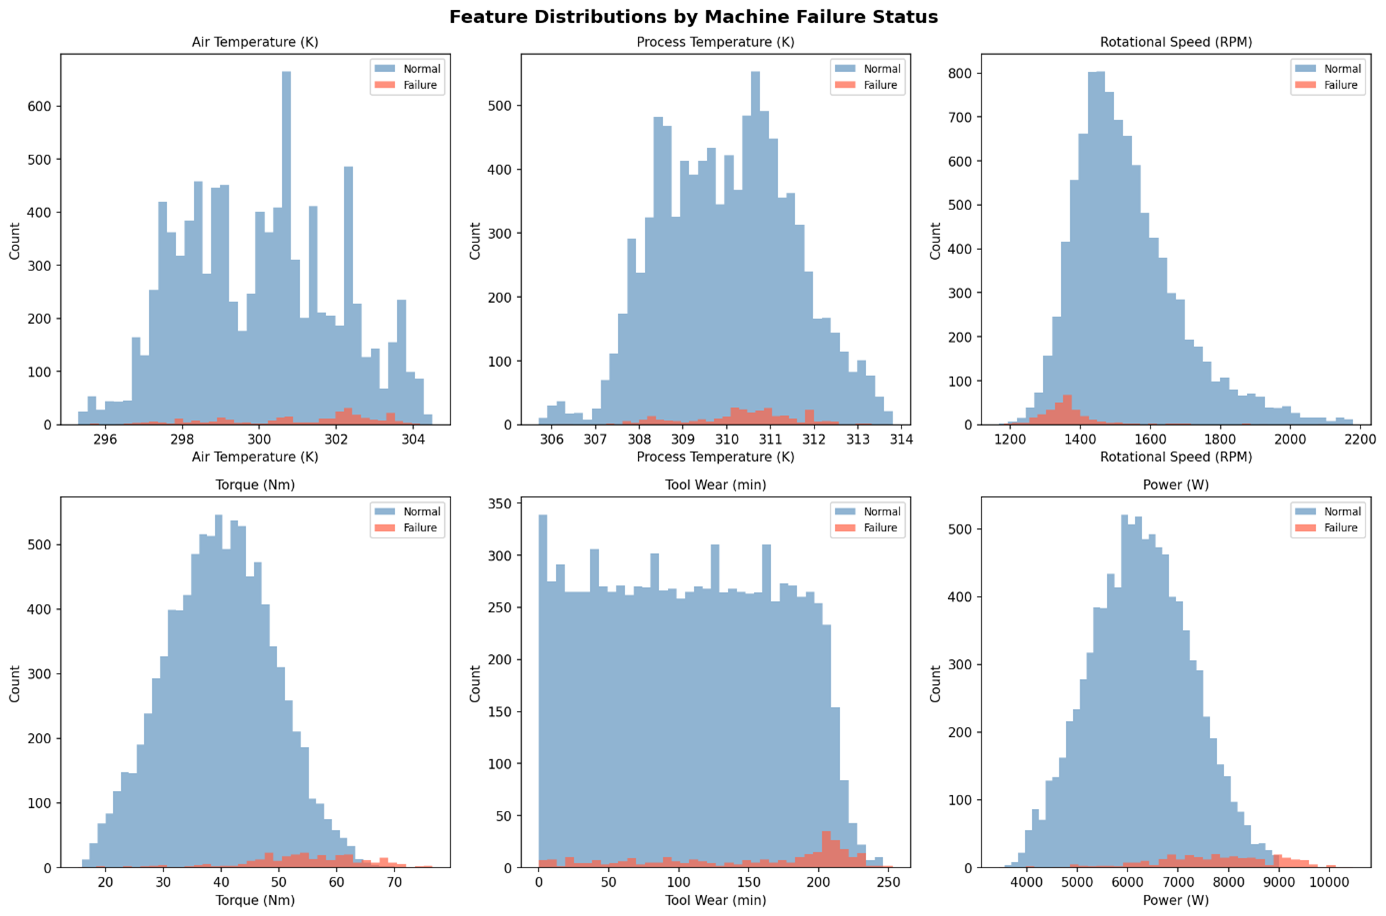
\includegraphics[width=0.8\textwidth]{1.png}
    \caption{Biểu đồ phân phối của các đặc trưng sau khi chuyển đổi}   
\end{figure}

\begin{figure}[H]
    \centering
    % Thay thế placeholder bằng tên file ảnh của bạn
    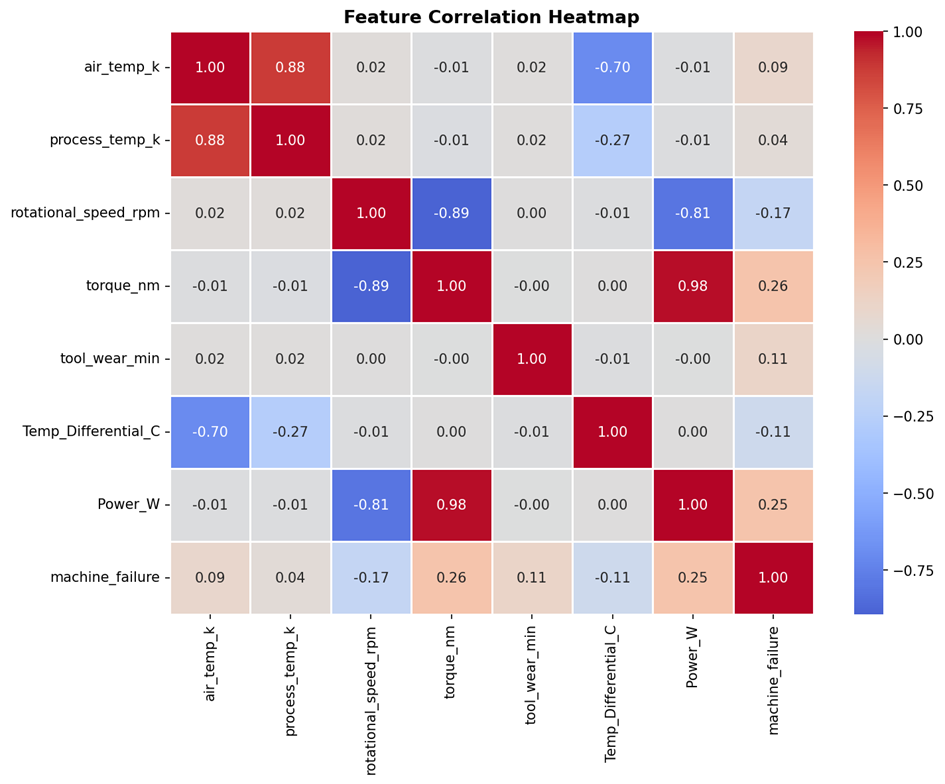
\includegraphics[width=0.8\textwidth]{2.png}
    \caption{Bản đồ nhiệt (Heatmap) thể hiện độ tương quan của các đặc trưng}
\end{figure}

\subsection{Chuyển đổi Dữ liệu}
Một số phép chuyển đổi theo đặc thù miền (domain-specific) đã được áp dụng để làm phong phú tập dữ liệu:
\begin{enumerate}
    \item \textbf{Chuyển đổi Nhiệt độ:} Nhiệt độ Không khí và Quá trình được chuyển đổi từ Kelvin sang độ C (trừ đi 273.15).
    \item \textbf{Khai phá Đặc trưng (Feature Engineering):} 
    \begin{itemize}
        \item \texttt{Temp\_Differential\_C}: Tính bằng Nhiệt độ Quá trình - Nhiệt độ Không khí.
        \item \texttt{Power\_W}: Công suất cơ học được tính bằng Mô-men xoắn và Tốc độ quay.
    \end{itemize}
    \item \textbf{Mã hóa Phân loại:} Cột \texttt{Type} (L, M, H) được mã hóa lần lượt thành 0, 1, 2.
    \item \textbf{Tạo Nhãn (Label Generation):} Một cột \texttt{Failure\_Type} duy nhất được suy ra từ các cờ lỗi nhị phân riêng lẻ (TWF, HDF, PWF, OSF, RNF).
\end{enumerate}





\section{Vùng Lưu trữ Tạm (Staging Area) và Đường ống ETL}

\subsection{Lưu trữ Cơ sở dữ liệu}
Một cơ sở dữ liệu PostgreSQL (\texttt{co4031\_dw}) đã được thiết lập. Một schema staging và một bảng phẳng \texttt{machine\_data} đã được tạo để chứa dữ liệu đã tiền xử lý trước khi tiến hành mô hình hóa chiều.

\begin{lstlisting}[language=SQL, caption= Staging Schema]
-- Create schema for staging area
CREATE SCHEMA IF NOT EXISTS staging;
DROP TABLE IF EXISTS staging.machine_data;

-- Create the staging table
CREATE TABLE staging.machine_data (
    record_id INTEGER PRIMARY KEY,
    product_id VARCHAR(20),
    quality_type CHAR(1),
    air_temp_k FLOAT,
    process_temp_k FLOAT,
    rotational_speed_rpm INTEGER,
    torque_nm FLOAT,
    tool_wear_min INTEGER,
    machine_failure SMALLINT,
    failure_twf SMALLINT,
    failure_hdf SMALLINT,
    failure_pwf SMALLINT,
    failure_osf SMALLINT,
    failure_rnf SMALLINT,
    -- Derived / transformed columns
    air_temp_c FLOAT,
    process_temp_c FLOAT,
    temp_differential_c FLOAT,
    power_w FLOAT,
    type_encoded SMALLINT,
    failure_type VARCHAR(50),
    load_timestamp TIMESTAMP DEFAULT CURRENT_TIMESTAMP
);

\end{lstlisting}


\begin{figure}[H]
    \centering
    % Thay thế placeholder bằng tên file ảnh của bạn
    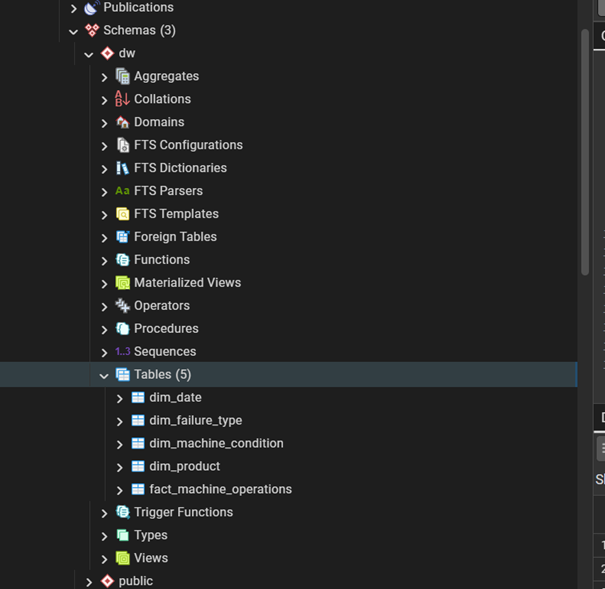
\includegraphics[width=0.8\textwidth]{staging.png}
    \caption{Tạo bảng staging trong PostgreSQL (pgAdmin)}
\end{figure}

\subsection{Triển khai ETL}
Quá trình ETL được thiết kế sử dụng hai phương pháp để đảm bảo tính linh hoạt:
\begin{itemize}
    \item \textbf{Tải bằng Python:} Một tập lệnh (\texttt{02\_load\_to\_dw.py}) sử dụng \texttt{SQLAlchemy} và \texttt{pandas.to\_sql} được phát triển để chèn hàng loạt dữ liệu CSV đã làm sạch trực tiếp vào bảng \texttt{staging.machine\_data}.
    \end{itemize}
    
\begin{lstlisting}[language=Python, Caption= Python ETL]
import pandas as pd
from sqlalchemy import create_engine, text
import warnings
warnings.filterwarnings('ignore')

# ============================================================
# CONNECTION CONFIGURATION
# ============================================================
# Change these if your PostgreSQL settings are different:
DB_USER = "postgres"
DB_PASSWORD = os.environ.get("DB_PASSWORD", "") # your PostgreSQL password
DB_HOST = "localhost"
DB_PORT = "5432"
DB_NAME = "co4031_dw"

CLEANED_PATH = r"C:\co4031_project\data\cleaned\machine_data_cleaned.csv"

# Build connection string
conn_str = f"postgresql+psycopg2://{DB_USER}:{DB_PASSWORD}@{DB_HOST}:{DB_PORT}/{DB_NAME}"

print("Connecting to PostgreSQL...")
engine = create_engine(conn_str)

# Test connection
with engine.connect() as conn:
    result = conn.execute(text("SELECT version()"))
    print(f"Connected! PostgreSQL version: {result.fetchone()[0][:30]}...")

# ============================================================
# LOAD DATA
# ============================================================

print("\nLoading cleaned CSV file...")
df = pd.read_csv(CLEANED_PATH)
print(f"Loaded {len(df)} rows, {len(df.columns)} columns.")

# Select and rename columns to match database table exactly
db_columns = [
    'record_id', 'product_id', 'quality_type',
    'air_temp_k', 'process_temp_k', 'rotational_speed_rpm',
    'torque_nm', 'tool_wear_min', 'machine_failure',
    'failure_twf', 'failure_hdf', 'failure_pwf',
    'failure_osf', 'failure_rnf',
    'Air_Temp_C', 'Process_Temp_C',
    'Temp_Differential_C', 'Power_W',
    'Type_Encoded', 'Failure_Type'
]

# Rename derived columns to lowercase for DB consistency
df = df.rename(columns={
    'Air_Temp_C': 'air_temp_c',
    'Process_Temp_C': 'process_temp_c',
    'Temp_Differential_C': 'temp_differential_c',
    'Power_W': 'power_w',
    'Type_Encoded': 'type_encoded',
    'Failure_Type': 'failure_type'
})

print("Loading data to staging.machine_data table...")

# Load using pandas to_sql (much faster than row-by-row INSERT)
df.to_sql(
    name='machine_data',
    schema='staging',
    con=engine,
    if_exists='replace', # 'replace' drops and recreates; use 'append' later
    index=False,
    chunksize=1000,      # process 1000 rows at a time
    method='multi'       # batch inserts (faster)
)

# Verify the load
with engine.connect() as conn:
    count = conn.execute(
        text("SELECT COUNT(*) FROM staging.machine_data")
    ).fetchone()[0]
    print(f"\nVerification: {count} rows loaded to staging.machine_data")

    # Show sample
    sample = conn.execute(
        text("SELECT record_id, quality_type, machine_failure, failure_type "
             "FROM staging.machine_data LIMIT 5")
    )
    print("\nSample rows:")
    for row in sample:
        print(f"ID={row[0]}, Type={row[1]}, Failure={row[2]}, Kind='{row[3]}'")

print("\n=== ETL LOAD COMPLETE ===")
\end{lstlisting}

\begin{itemize}    
    \item \textbf{Pentaho Data Integration (Spoon):} Một đường ống ETL trực quan (\texttt{machine\_etl.ktr}) đã được xây dựng. Các bước của đường ống bao gồm:
    \begin{enumerate}
        \item \textit{CSV file input}: Đọc dữ liệu thô.
        \item \textit{Filter rows}: Lọc các bản ghi không hợp lệ (ví dụ: Tốc độ quay $>$ 0).
        \item \textit{Calculator}: Chuẩn hóa nhiệt độ sang độ C và tính toán Chênh lệch Nhiệt độ và Công suất.
        \item \textit{Value Mapper}: Mã hóa loại chất lượng.
        \item \textit{Modified JavaScript Value}: Một tập lệnh để gộp các cờ lỗi thành một \texttt{failure\_type} dễ đọc.
        \item \textit{Table output}: Đẩy luồng dữ liệu đã chuyển đổi vào bảng staging của PostgreSQL.
    \end{enumerate}
\end{itemize}


\begin{figure}[H]
    \centering
    % Thay thế placeholder bằng tên file ảnh của bạn
    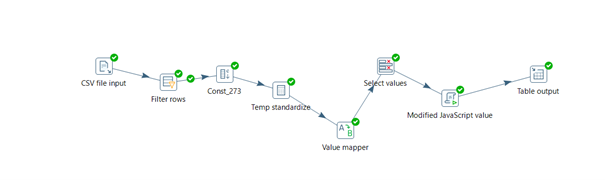
\includegraphics[width=0.75\linewidth]{3.png}
    \caption{Quy trình ETL trực quan trên Pentaho Data Integration}
\end{figure}

\begin{figure}[H]
    \centering
    % Thay thế placeholder bằng tên file ảnh của bạn
    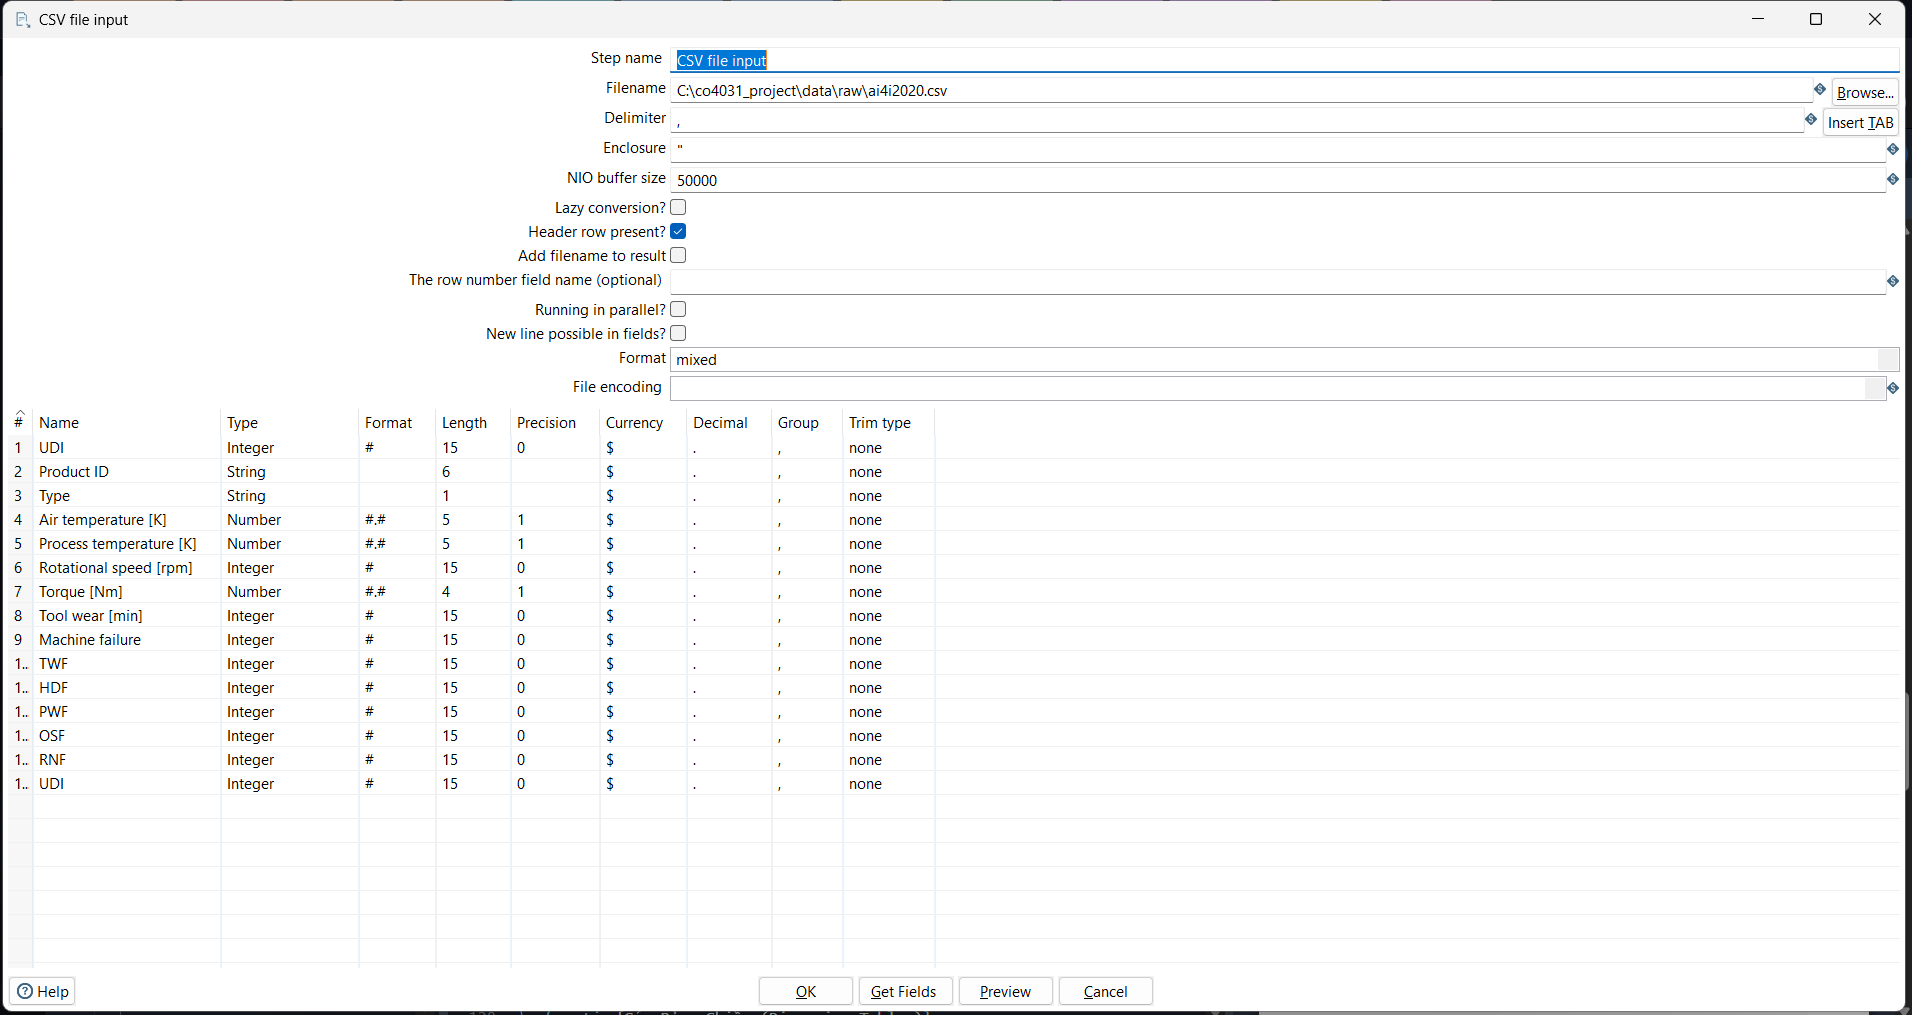
\includegraphics[width=0.8\textwidth]{etl 1.png}
    \caption{Bước 1}
\end{figure}
\begin{figure}[H]
    \centering
    % Thay thế placeholder bằng tên file ảnh của bạn
    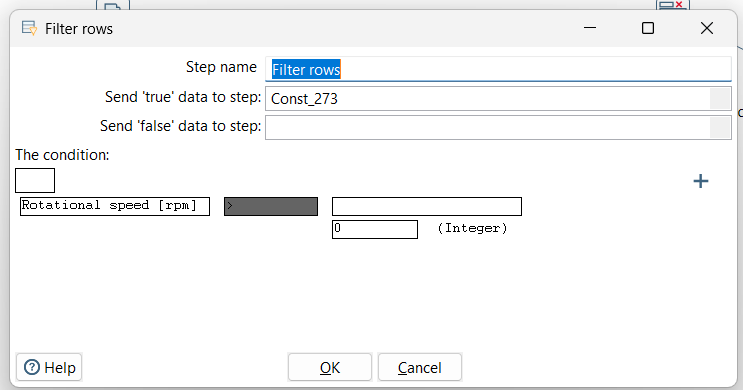
\includegraphics[width=0.8\textwidth]{etl 2.png}
    \caption{Bước 2}
\end{figure}
\begin{figure}[H]
    \centering
    % Thay thế placeholder bằng tên file ảnh của bạn
    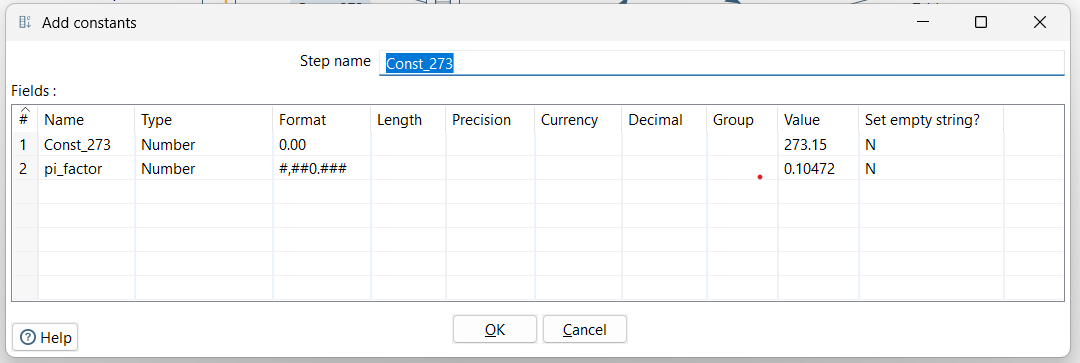
\includegraphics[width=0.8\textwidth]{etl 3.png}
    \caption{Bước 3}
\end{figure}
\begin{figure}[H]
    \centering
    % Thay thế placeholder bằng tên file ảnh của bạn
    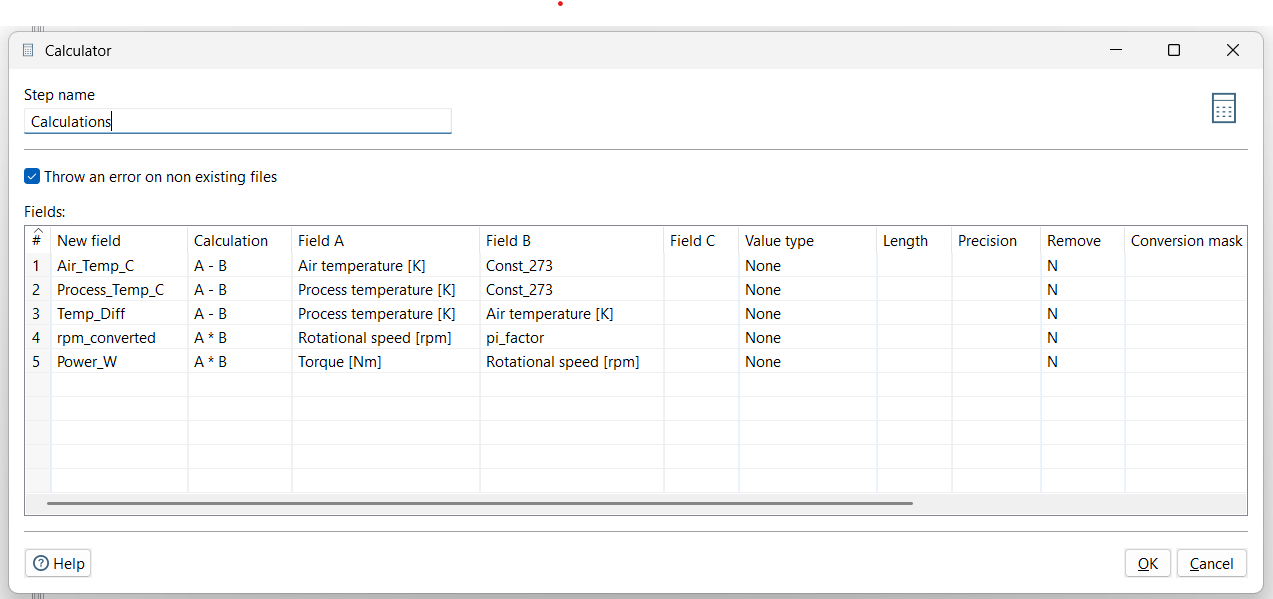
\includegraphics[width=0.8\textwidth]{etl 4.png}
    \caption{Bước 4}
\end{figure}
\begin{figure}[H]
    \centering
    % Thay thế placeholder bằng tên file ảnh của bạn
    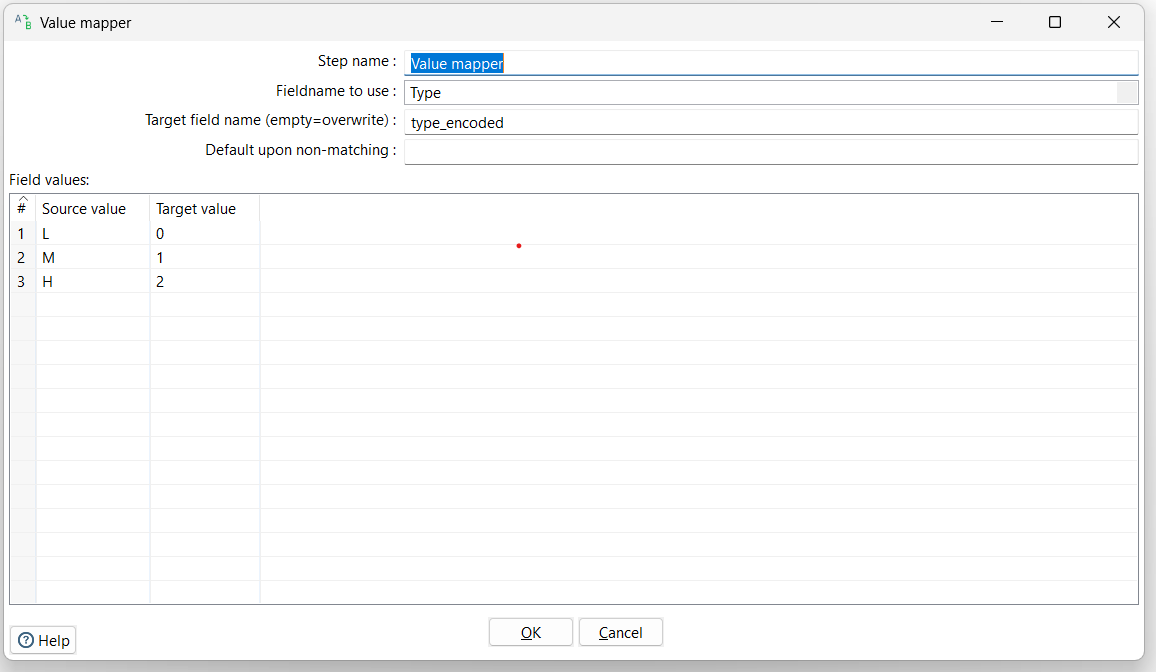
\includegraphics[width=0.8\textwidth]{etl 5.png}
    \caption{Bước 5}
\end{figure}
\begin{figure}[H]
    \centering
    % Thay thế placeholder bằng tên file ảnh của bạn
    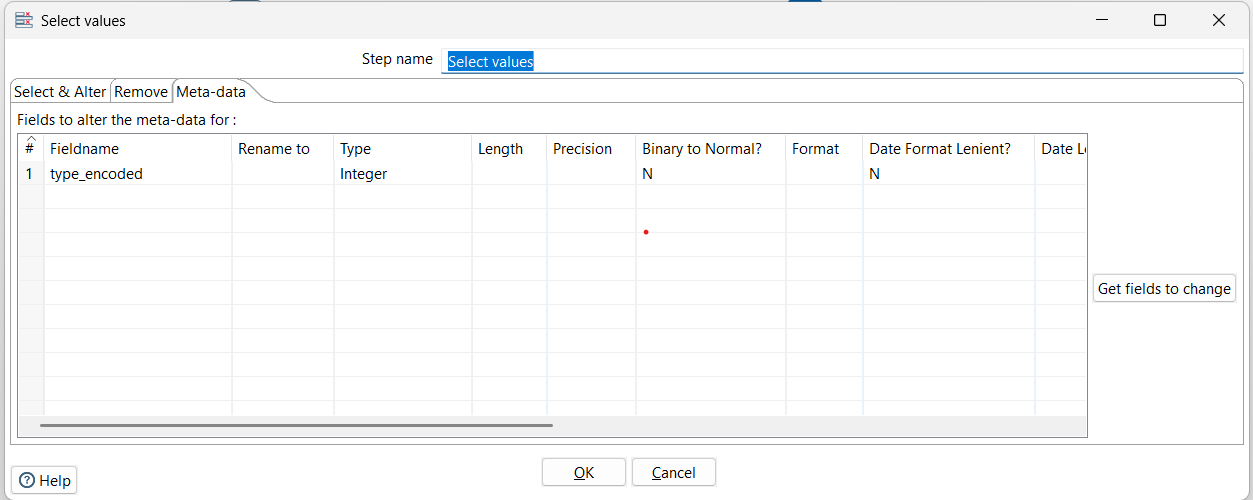
\includegraphics[width=0.8\textwidth]{etl 6.png}
    \caption{Bước 6}
\end{figure}
\begin{figure}[H]
    \centering
    % Thay thế placeholder bằng tên file ảnh của bạn
    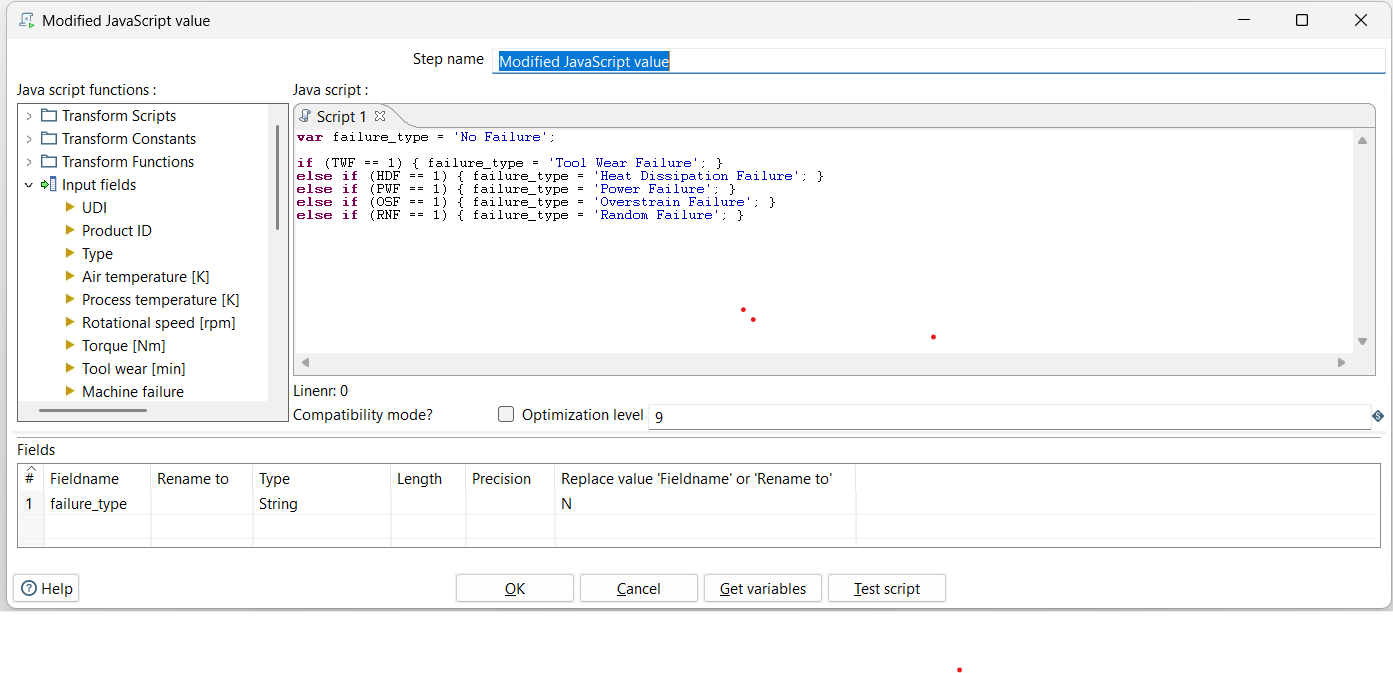
\includegraphics[width=0.8\textwidth]{etl 7.png}
    \caption{Bước 7}
\end{figure}
\begin{figure}[H]
    \centering
    % Thay thế placeholder bằng tên file ảnh của bạn
    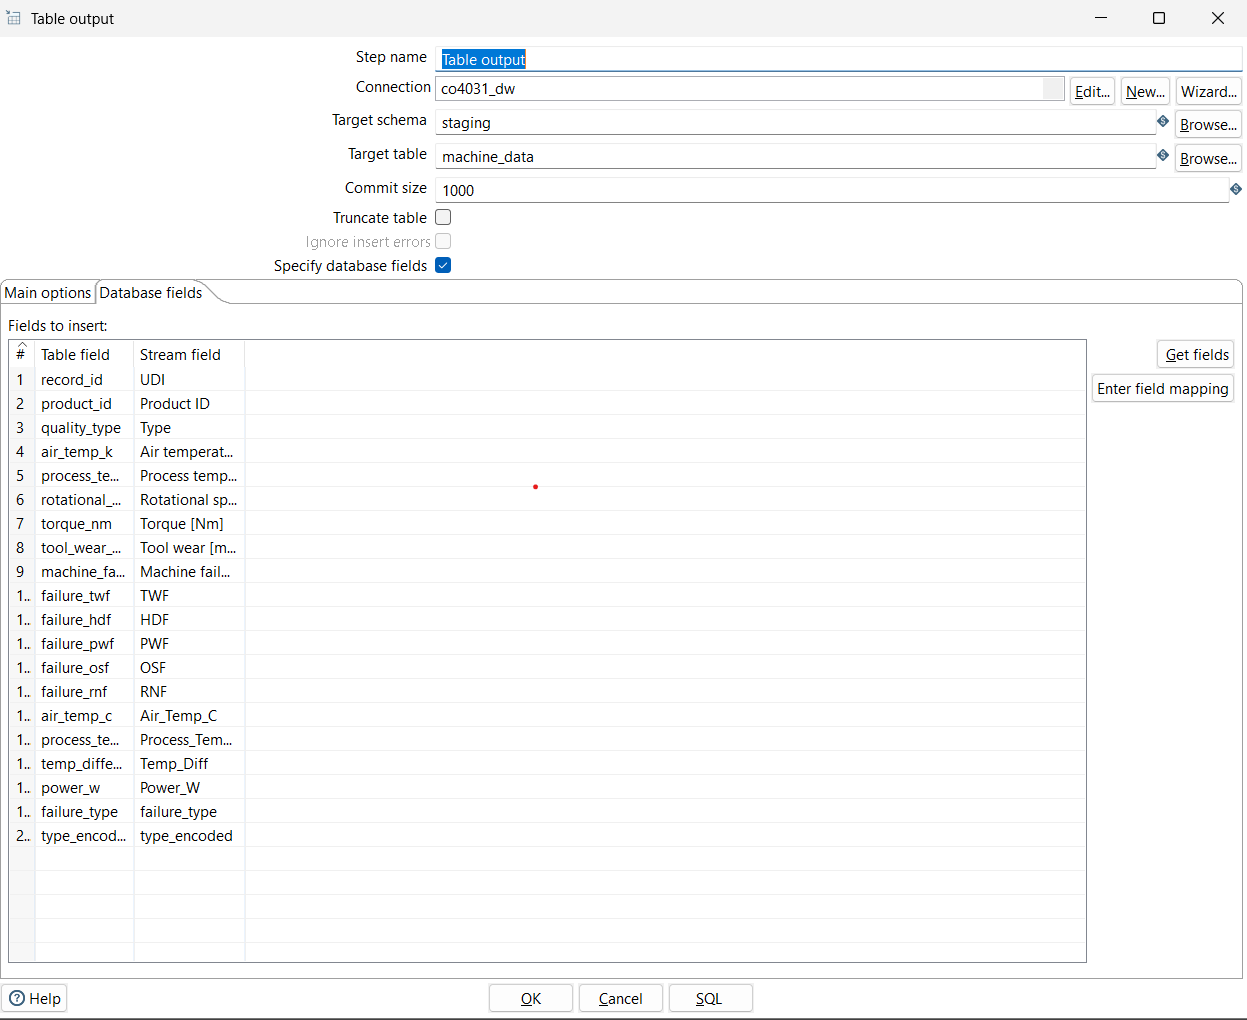
\includegraphics[width=0.8\textwidth]{etl 8.png}
    \caption{Bước 8}
\end{figure}

\begin{figure}[H]
    \centering
    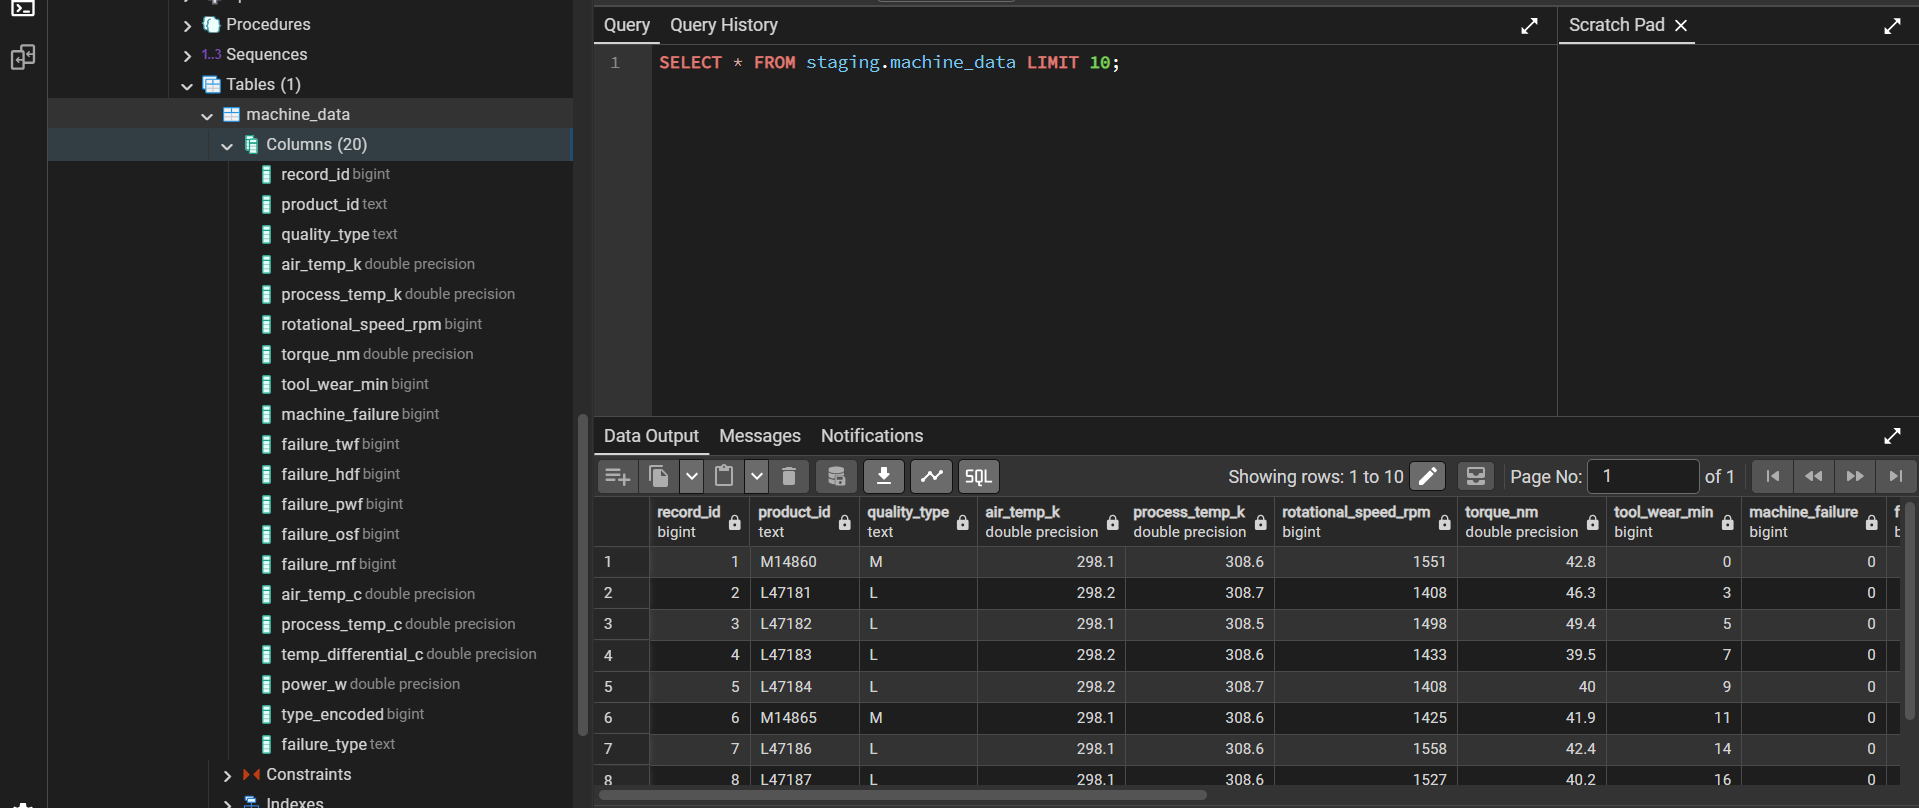
\includegraphics[width=0.75\linewidth]{factsql.png}
    \caption{Sau khi populate dữ liệu vào staging}
\end{figure}

\section{Thiết kế Kho Dữ Liệu: Lược đồ Hình sao (Star Schema)}
Để hỗ trợ hiệu quả các truy vấn OLAP, dữ liệu phẳng trong vùng staging được mô hình hóa thành một Lược đồ Hình sao bao gồm một bảng sự kiện (fact table) và bốn bảng chiều (dimension tables).


\begin{figure}[H]
    \centering
    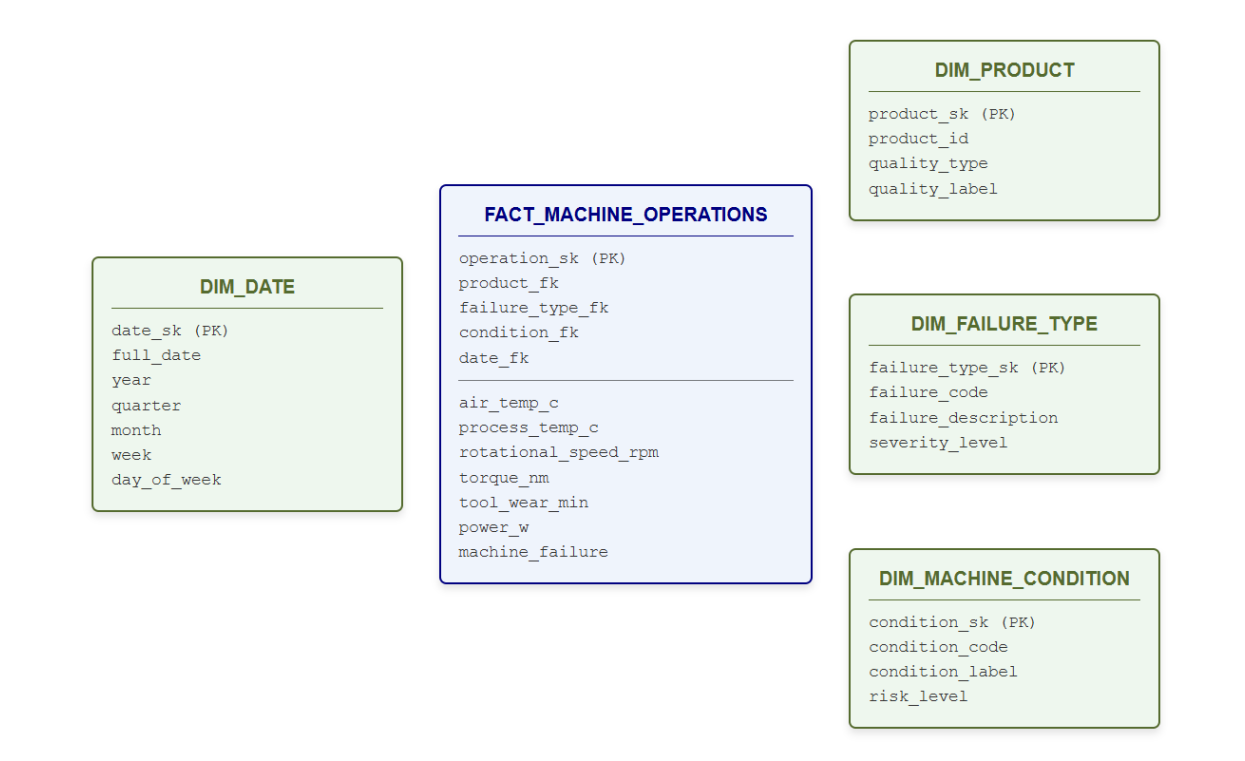
\includegraphics[width=0.75\linewidth]{star.png}
    \caption{Lược đồ Hình sao cho Kho Dữ liệu Sản xuất}
\end{figure}



\subsection{Các Bảng Chiều (Dimension Tables)}
\begin{itemize}
    \item \textbf{DIM\_DATE}: Chứa cấu trúc phân cấp thời gian (Năm, Quý, Tháng, Tuần). Vì dữ liệu thô thiếu dấu thời gian, một mô phỏng đã phân bổ các hoạt động qua các ngày làm việc trong năm 2023.
    \item \textbf{DIM\_PRODUCT}: Lưu trữ các cấp chất lượng sản phẩm (Thấp, Trung bình, Cao).
    \item \textbf{DIM\_FAILURE\_TYPE}: Phân loại lỗi (ví dụ: Lỗi mòn dao cụ, Lỗi tản nhiệt) cùng với mức độ nghiêm trọng (từ 1 đến 3).
    \item \textbf{DIM\_MACHINE\_CONDITION}: Phân loại sức khỏe máy dựa trên số phút mòn của dao cụ (Dao mới, Dao ở giữa vòng đời, Dao cũ, Dao bị mòn) và gán mức độ rủi ro.
\end{itemize}

\subsection{Bảng Sự kiện (Fact Table)}
\textbf{FACT\_MACHINE\_OPERATIONS} nằm ở trung tâm của lược đồ. Nó chứa các khóa ngoại (foreign keys) liên kết tới các chiều đã nêu ở trên và lưu trữ các số đo liên tục như \texttt{air\_temp\_c}, \texttt{process\_temp\_c}, \texttt{torque\_nm}, \texttt{tool\_wear\_min}, và \texttt{power\_w}. Bảng này cũng lưu trữ các cờ lỗi nhị phân.

\begin{lstlisting}[language=Python, Caption= Python nhập dữ liệu vào Schema]
import pandas as pd
from sqlalchemy import create_engine, text
import numpy as np
from datetime import date, timedelta
import random
import warnings

warnings.filterwarnings('ignore')

# ============================================================
# CONNECTION CONFIGURATION
# ============================================================
DB_USER = "postgres"
DB_PASSWORD = os.environ.get("DB_PASSWORD", "") # Update this to your actual password!
DB_HOST = "localhost"
DB_PORT = "5432"
DB_NAME = "co4031_dw"

conn_str = f"postgresql+psycopg2://{DB_USER}:{DB_PASSWORD}@{DB_HOST}:{DB_PORT}/{DB_NAME}"
engine = create_engine(conn_str)

print("Loading staging data...")
df = pd.read_sql("SELECT * FROM staging.machine_data", engine)
print(f"Loaded {len(df)} rows from staging.")

# ============================================================
# POPULATE DIM_PRODUCT
# ============================================================
print("\nPopulating dim_product ...")

quality_label_map = {
    'L': 'Low Quality',
    'M': 'Medium Quality',
    'H': 'High Quality'
}
quality_tier_map = {'L': 1, 'M': 2, 'H': 3}

products = df[['product_id', 'quality_type']].drop_duplicates()
products['quality_label'] = products['quality_type'].map(quality_label_map)
products['quality_tier'] = products['quality_type'].map(quality_tier_map)

with engine.connect() as conn:
    conn.execute(text("DELETE FROM dw.dim_product"))
    conn.commit()

products.to_sql('dim_product', schema='dw', con=engine, if_exists='append', index=False)
print(f"Inserted {len(products)} product records.")

# Fetch back product SK mapping
dim_prod_df = pd.read_sql("SELECT product_sk, product_id FROM dw.dim_product", engine)
prod_map = dict(zip(dim_prod_df['product_id'], dim_prod_df['product_sk']))

# ============================================================
# POPULATE DIM_FAILURE_TYPE (already populated via SQL)
# ============================================================
dim_fail_df = pd.read_sql("SELECT failure_type_sk, failure_code FROM dw.dim_failure_type", engine)
fail_code_map = dict(zip(dim_fail_df['failure_code'], dim_fail_df['failure_type_sk']))

def get_failure_code(row):
    if row['failure_twf'] == 1: return 'TWF'
    if row['failure_hdf'] == 1: return 'HDF'
    if row['failure_pwf'] == 1: return 'PWF'
    if row['failure_osf'] == 1: return 'OSF'
    if row['failure_rnf'] == 1: return 'RNF'
    return 'NF'

df['failure_code'] = df.apply(get_failure_code, axis=1)
df['failure_type_fk'] = df['failure_code'].map(fail_code_map)

# ============================================================
# POPULATE DIM_MACHINE_CONDITION
# ============================================================
dim_cond_df = pd.read_sql("SELECT condition_sk, condition_code FROM dw.dim_machine_condition", engine)
cond_map = dict(zip(dim_cond_df['condition_code'], dim_cond_df['condition_sk']))

def get_condition_code(wear_min):
    if wear_min <= 100: return 'NEW_TOOL'
    if wear_min <= 200: return 'MID_TOOL'
    if wear_min <= 240: return 'OLD_TOOL'
    return 'WORN_TOOL'

df['condition_code'] = df['tool_wear_min'].apply(get_condition_code)
df['condition_fk'] = df['condition_code'].map(cond_map)

# ============================================================
# SIMULATE DATES (since dataset has no timestamps)
# ============================================================
# We assign records to business days in 2023, simulating 10,000 operations
random.seed(42)
start_date = date(2023, 1, 2)
all_biz_days = []
d = start_date
while len(all_biz_days) < 400: # Ensure enough days
    if d.weekday() < 5: # Monday-Friday
        all_biz_days.append(d)
    d += timedelta(days=1)

assigned_dates = [random.choice(all_biz_days) for _ in range(len(df))]
df['simulated_date'] = assigned_dates

# Fetch date dimension SK map
dim_date_df = pd.read_sql("SELECT date_sk, full_date FROM dw.dim_date", engine)
dim_date_df['full_date'] = pd.to_datetime(dim_date_df['full_date']).dt.date
date_map = dict(zip(dim_date_df['full_date'], dim_date_df['date_sk']))
df['date_fk'] = df['simulated_date'].map(date_map)

# ============================================================
# POPULATE FACT TABLE
# ============================================================
print("\nPopulating fact_machine_operations ...")

df['product_fk'] = df['product_id'].map(prod_map)

fact_cols = [
    'product_fk', 'failure_type_fk', 'condition_fk', 'date_fk',
    'record_id', # this will become source_record_id
    'air_temp_c', 'process_temp_c', 'temp_differential_c', 
    'rotational_speed_rpm', 'torque_nm', 'tool_wear_min', 'power_w',
    'machine_failure', 'failure_twf', 'failure_hdf', 'failure_pwf',
    'failure_osf', 'failure_rnf'
]

# Create fact dataframe and rename the source tracking ID
fact_df = df[fact_cols].copy()
fact_df = fact_df.rename(columns={'record_id': 'source_record_id'})

# Drop nulls in FKs (safety check)
before = len(fact_df)
fact_df = fact_df.dropna(subset=['product_fk', 'failure_type_fk', 'condition_fk', 'date_fk'])
dropped = before - len(fact_df)
if dropped > 0:
    print(f"Warning: dropped {dropped} rows with null FK values")

# Load to fact table
with engine.connect() as conn:
    conn.execute(text("DELETE FROM dw.fact_machine_operations"))
    conn.commit()

fact_df.to_sql('fact_machine_operations', schema='dw', con=engine, if_exists='append', index=False, chunksize=500, method='multi')

# Verify
with engine.connect() as conn:
    cnt = conn.execute(text("SELECT COUNT(*) FROM dw.fact_machine_operations")).fetchone()[0]
    print(f"Inserted {cnt} rows into fact_machine_operations.")
    
    fail_cnt = conn.execute(text("SELECT COUNT(*) FROM dw.fact_machine_operations WHERE machine_failure = 1")).fetchone()[0]
    print(f"Of which {fail_cnt} are failure records.")

print("\n=== STAR SCHEMA POPULATION COMPLETE ===")

\end{lstlisting}

\begin{figure}[H]
    \centering
    % Thay thế placeholder bằng tên file ảnh của bạn
    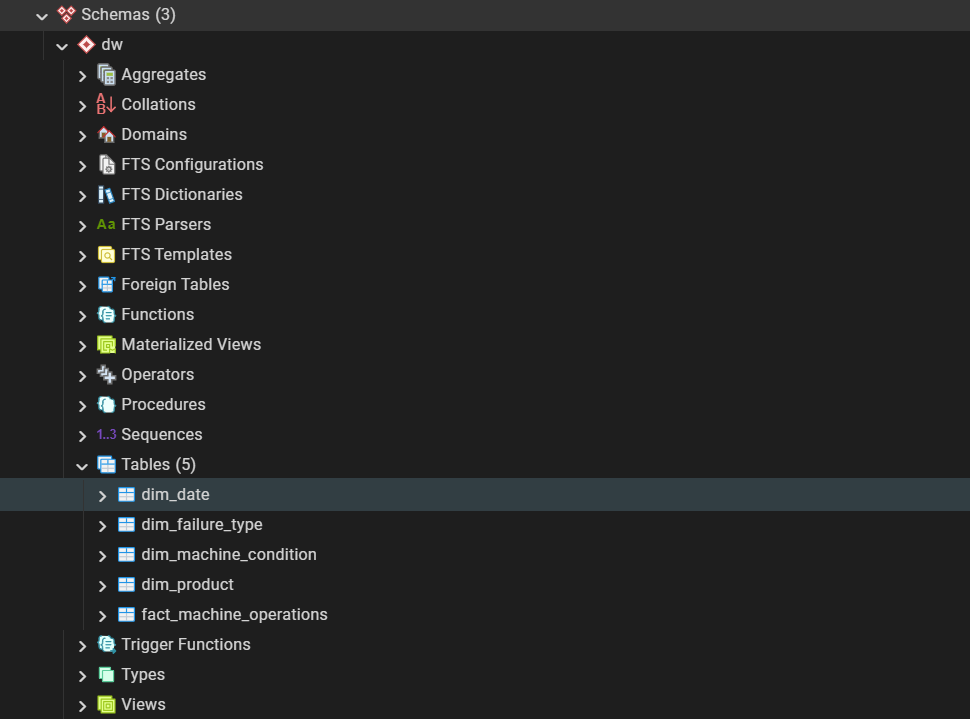
\includegraphics[width=0.75\linewidth]{schema1.png}
    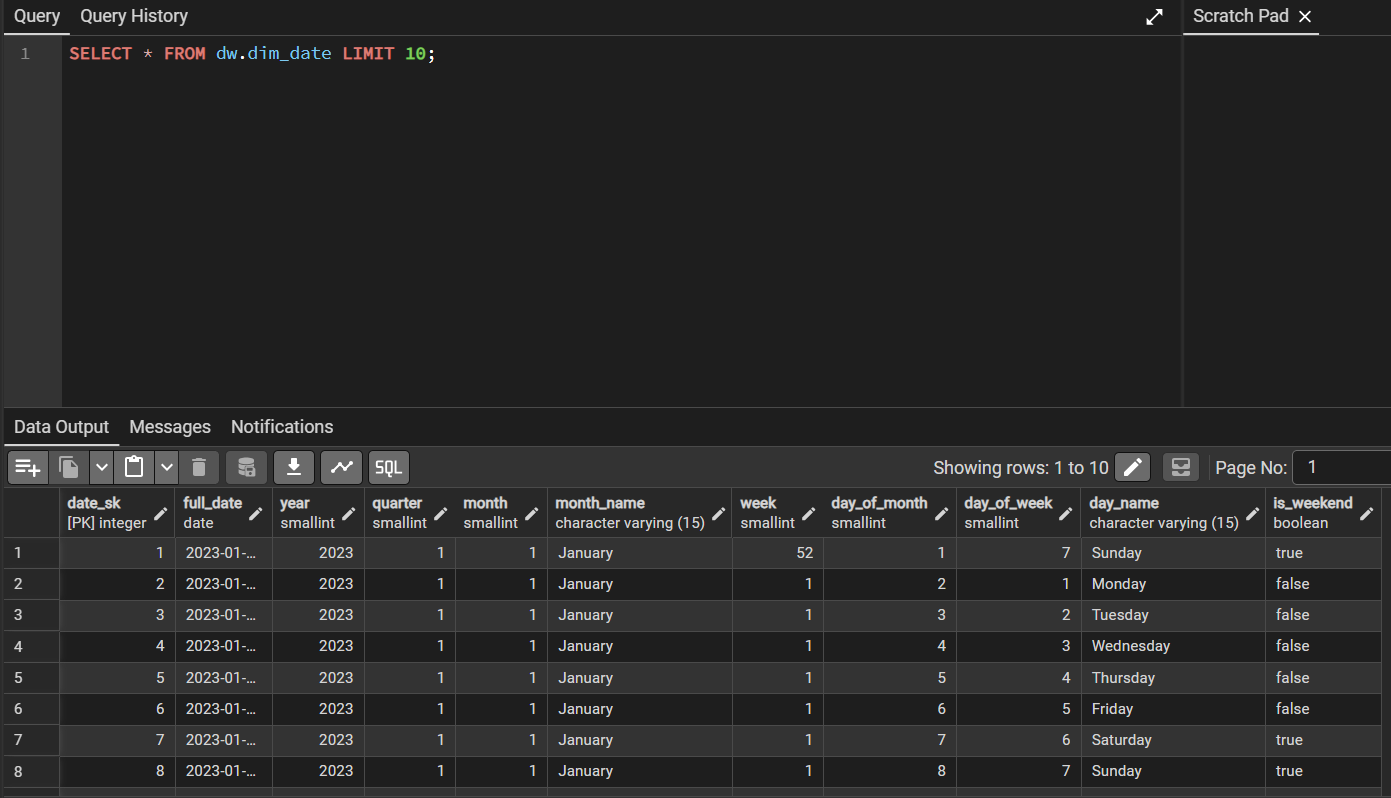
\includegraphics[width=0.75\linewidth]{schema2.png}
    \caption{Dữ liệu đã được nạp thành công vào Schema}
\end{figure}


\section{Phân tích OLAP}
Với Lược đồ Hình sao đã được nạp dữ liệu, một số truy vấn OLAP đã được phát triển để trích xuất thông tin tình báo kinh doanh.

\subsection{Truy vấn 1: Tỷ lệ Lỗi theo Loại Chất lượng Sản phẩm}
Phân tích độ tin cậy của các cấp chất lượng sản phẩm khác nhau (L, M, H) bằng cách tính tổng số hoạt động, tỷ lệ lỗi, mô-men xoắn trung bình và độ mòn trung bình của dao cụ cho mỗi cấp.

\begin{figure}[H]
    \centering
    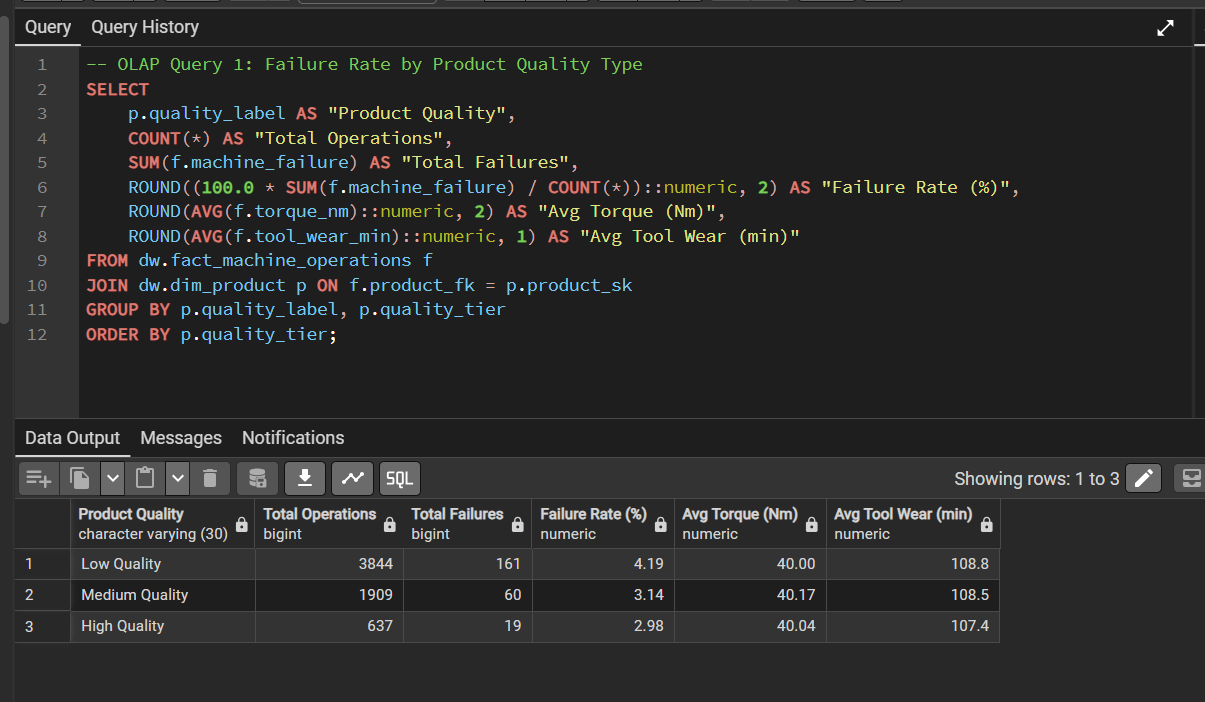
\includegraphics[width=0.75\linewidth]{olaf1.png}
    \caption{Tỷ lệ Lỗi theo Loại Chất lượng Sản phẩm}
\end{figure}

\subsection{Truy vấn 2: Xu hướng Lỗi Hàng tháng}
Sử dụng bảng \texttt{DIM\_DATE} để nhóm các hoạt động theo năm và tháng. Truy vấn này tính toán tỷ lệ lỗi hàng tháng, cung cấp cái nhìn rõ ràng về các sai lệch hoạt động có thể xảy ra theo mùa hoặc theo thời gian.

\begin{figure}[H]
    \centering
    % Thay thế placeholder bằng tên file ảnh của bạn
    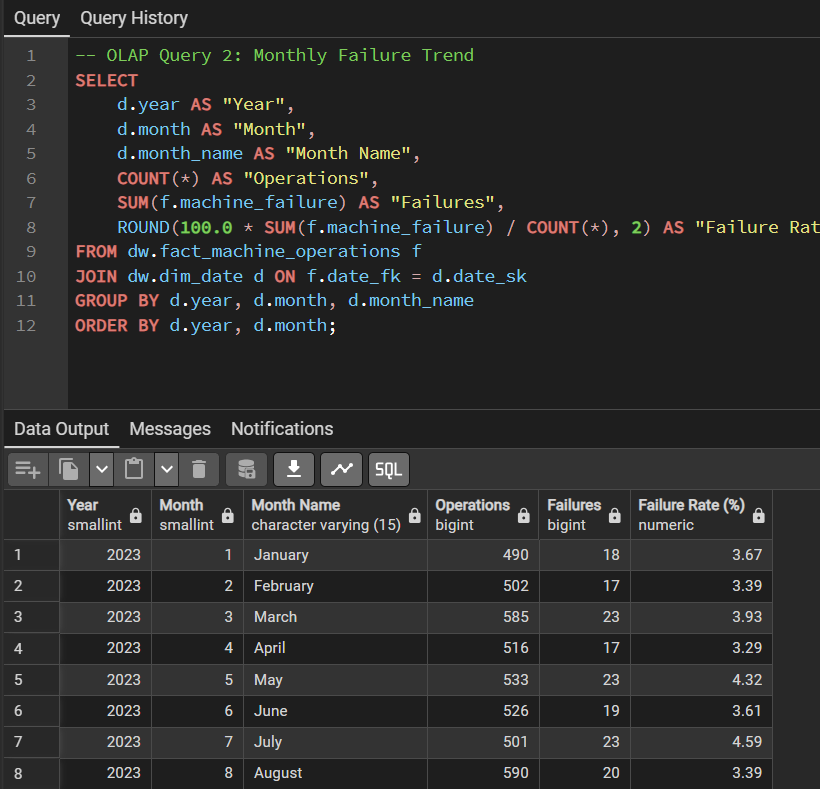
\includegraphics[width=0.75\linewidth]{olaf2.png}
    \caption{Kết quả truy vấn xu hướng lỗi hàng tháng}
\end{figure}

\subsection{Truy vấn 3: Phân phối Lỗi theo Loại Lỗi}
Tổng hợp dữ liệu theo các danh mục lỗi được định nghĩa trong \texttt{DIM\_FAILURE\_TYPE}. Truy vấn này tính toán số lần xuất hiện và tỷ lệ phần trăm trên tổng số lỗi, làm nổi bật xem lỗi cơ học, lỗi nhiệt, hay lỗi điện là phổ biến nhất.
\begin{figure}[H]
    \centering
    % Thay thế placeholder bằng tên file ảnh của bạn
    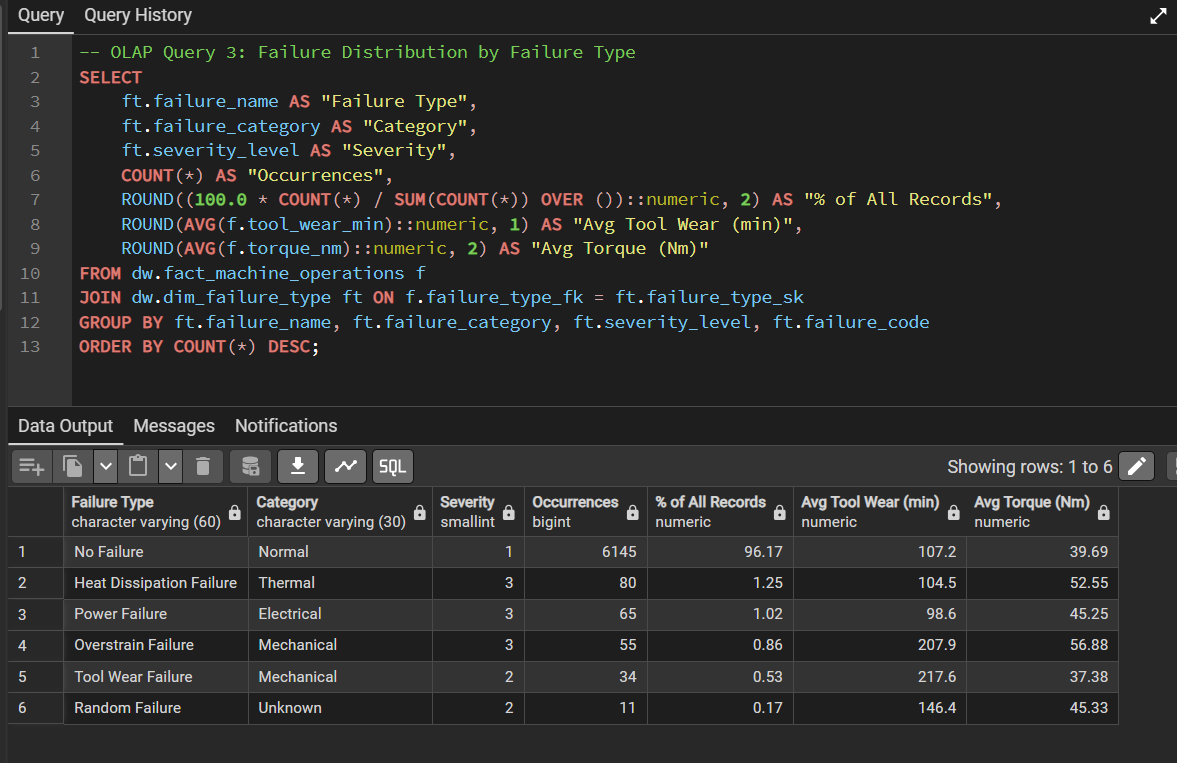
\includegraphics[width=0.75\linewidth]{olaf3.png}    \caption{Kết quả truy vấn xu hướng lỗi hàng tháng}
\end{figure}

\subsection{Truy vấn 4: Tình trạng Máy vs Tỷ lệ Lỗi}
Sử dụng bảng \texttt{DIM\_MACHINE\_CONDITION} để đánh giá xem tuổi của dao cụ ảnh hưởng như thế nào đến xác suất xảy ra lỗi. Truy vấn vạch ra các hoạt động trên nhiều mức độ rủi ro khác nhau (Thấp, Trung bình, Cao, Nghiêm trọng) và liên kết chúng với các đề xuất bảo trì có thể hành động.
\begin{figure}[H]
    \centering
    % Thay thế placeholder bằng tên file ảnh của bạn
    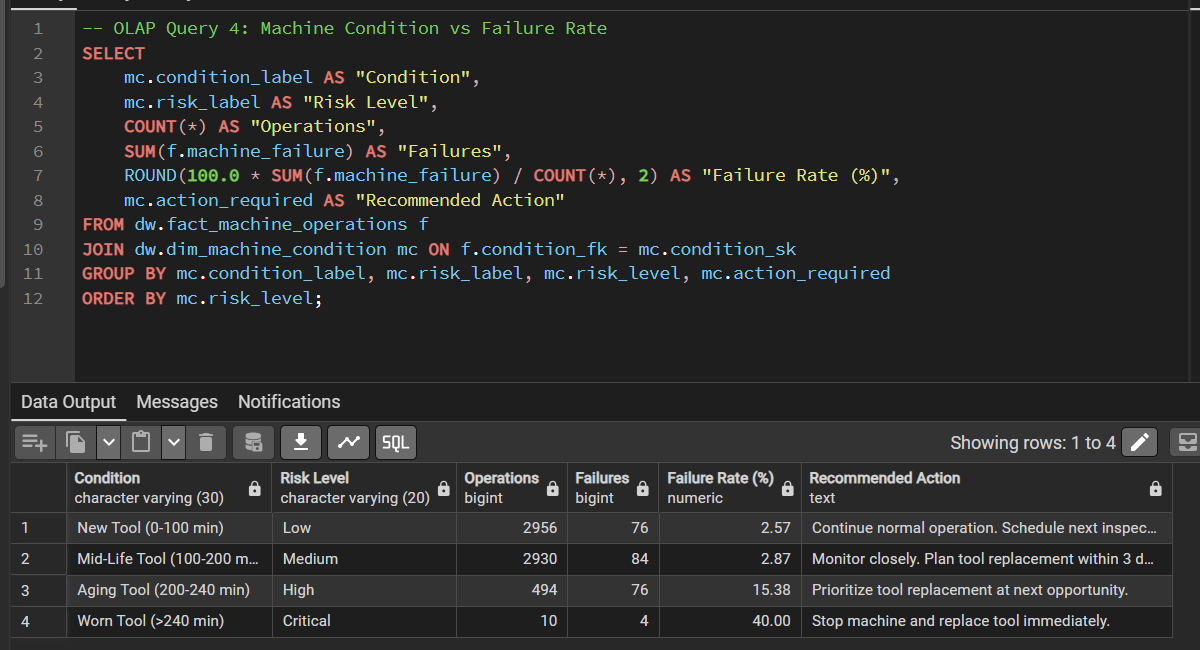
\includegraphics[width=0.75\linewidth]{olaf4.png}
    \caption{Kết quả truy vấn xu hướng lỗi hàng tháng}
\end{figure}


\section{Kết luận}
Dự án đã chuyển đổi thành công dữ liệu cảm biến máy thô thành một Kho dữ liệu có cấu trúc, tối ưu cho truy vấn. Việc triển khai các bước tiền xử lý mạnh mẽ, một đường ống ETL có hệ thống (qua Python và Pentaho), và mô hình hóa chiều cho phép theo dõi sức khỏe máy hiệu quả và phân tích bảo trì dự đoán thông qua các truy vấn OLAP toàn diện.

\end{document}
